\documentclass[a4paper,12pt]{article}

\title{EMBS Summer Assessment Report}
\author{Y8143160}

\usepackage{graphicx}
\usepackage[table]{xcolor}


\setcounter{tocdepth}{1}
\setcounter{secnumdepth}{2}

\newcommand{\todo}[1]{\textcolor{red}{[TODO: #1]}}


\begin{document}

\maketitle

\begin{center}
  983 words, per \texttt{M-x tex-count-words}
\end{center}

\section{Design}

Looking at the problem statement, it was pretty clear that there is no
(easy) closed-form solution or obvious straight-line algorithm to
solve the tiling problem. This suggested some kind of vaguely
brute-force approach to exploring the search space to find valid
tilings.

I started by considering a few of the obvious approaches to this kind
of problem:

\begin{itemize}
\item Tree search of the state space
\item Hill climbing
\item Genetic algorithms
\item Composing solutions from smaller valid tilings (i.e., $1 \times
  1$ tiles $\rightarrow$ $2 \times 1$ tiles $\rightarrow$ $2 \times 2$
  tiles, etc).
\end{itemize}

A couple of considerations are immediately apparent:

\begin{itemize}
\item Resources (especially memory) on the target platform are very
  limited.
\item Both back-of-the-envelope calculations and the problem statement
  itself suggested that a large amount of the calculation would have
  to happen in a custom hardware component to achieve reasonable
  performance.
\end{itemize}

Memory limitations and the difficulty of devising a suitable fitness
function immediately knock out hill-climbing and genetic
algorithms. Some kind of divide-and-conquer or `composition of smaller
blocks' approach is always appealing, but probably a dead end here
because of the structure of the problem, the memory required to store
the various components, and the unsuitability of the necessary fancy
data structures for custom hardware. So we're left with some variation
of tree search.

Not wishing to outsmart myself from the outset, I determined to
evaluate the performance of the obvious naive tree search before
trying to be tricky. Depth-first search is cheaper (or more easily
cheap) from a memory point of view, so that is where I started.

The natural way to fit depth-first search to this problem is to
stipulate that adding or removing nodes outright corresponds to moving
down or up the tree, and rotating or replacing the most-recent node
corresponds to moving left or right between sibling nodes.

\begin{figure}
  
  \begin{center}
    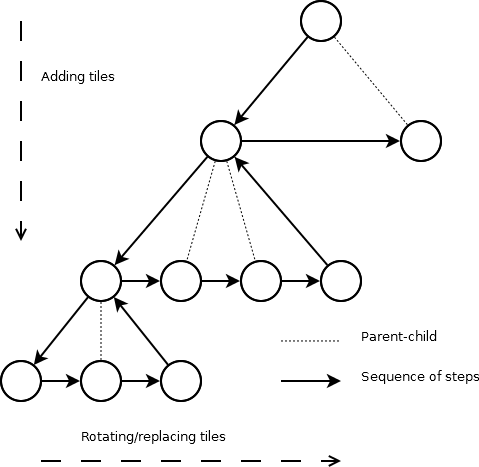
\includegraphics[scale=0.5]{tree}
    \caption{Correspondence between tile placement and the search tree}
  \end{center}
  
\end{figure}

Serendipitously, this approach has a natural and memory-efficient
representation as an array of pairs $(tile, rotation)$. Denoting tiles
by sequential indices, and knowing the number of distinct rotations,
it is easy to determine the next or previous sibling of a node in this
implicit tree representation.

This representation also has a rather fetching mechanical
visualisation as a carousel of tiles, the edges of which are carried
on epicycles; the whole whirling along a row of tiles forming a
partial solution, \textit{viz}:

\begin{figure}
  
  \begin{center}
    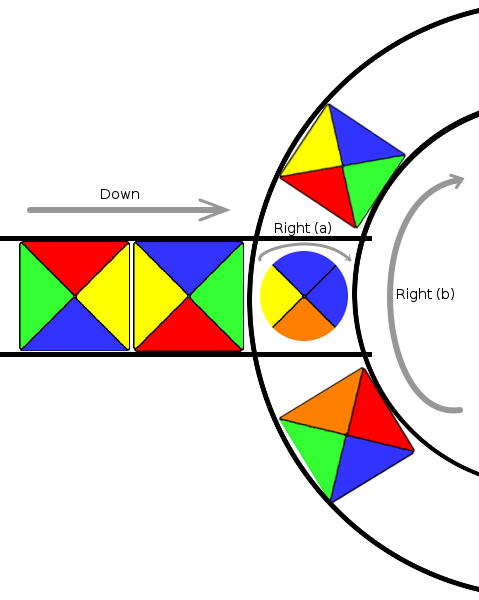
\includegraphics[scale=0.3]{spinner}
    \caption{The implicit tree structure used by the program}
  \end{center}
  
\end{figure}

\section{Implementation}

\subsection{Prototyping}

The solver was prototyped off-target as a command-line C program. This
gave a conveniently short development feedback cycle, as well as the
advantages of a powerful desktop processor and good debugging tools. A
range of small command-line programs to generate, shuffle, and
visualise (in glorious ANSI technicolour) tilesets formed a convenient
testbench upon which to prototype and evaluate various approaches and
optimisations.

I took the unscientific, but ultimately justified, hypothesis that the
performance of straight C on a desktop processor would be comparable
(within some small factor) to optimised custom hardware on a small
FPGA. This provided a useful reference point to assess progress on
algorithm development.

The algorithm as prototyped was basically depth-first search with
implict tree as outlined above. The only real optimisation introduced
at this stage was to use a lookup table from colours to bitmask sets
to efficiently filter out tiles which had no chance of being a
suitable candidate: this gave a speedup of roughly an order of
magnitude. At this point, solving most $6 \times 6$, 10-colour puzzles
took a typical desktop machine a few tens to a few hundreds of
milliseconds; by the heuristic above, this was deemed
adequate. (Obviously, the nature of the search means that pathological
examples can take quite a few orders of magnitude longer).

\subsection{On-Target Development}

The VGA and Ethernet components are largely unrevolutionary: the VGA
has a little trickiness whereby it spends most of its time looking
like QVGA for maximum convenience (this also gives us striped
`colours' for free), but otherwise a join-the-dots exercise.

The whole tile-solver component was turned wholesale into a single
Vivado HLS component. As the whole component exists to manipulate the
search tree, this became a piece of global state, with `instructions'
such as \texttt{down()}, \texttt{up()}, and \texttt{right()}, to
manipulate it.
\footnote{For reasons of exposition, this is mentioned here, but
  obviously this structure was present in the prototype. Converting
  the prototype to an HLS component consisted largely in replacing
  \texttt{scanf()} with \texttt{axi\_stream::read()}}.
Notwithstanding the stigma attached to global state, this proved
pleasantly readable, and required little tuning to compile reasonably
well: taking advantage of arbitrary-precision integers to narrow the
more obvious types was sufficient to produce a component small enough
to fit alongside the other components and (to my great delight) meet
the aforementioned performance obligations.

The tile-solver was augmented further to allow commands and responses
sent back and forth across the AXI streams to abort and restart
solving, and trigger extra backtracking to search for more than one
solution. This makes it straightforward to page through all of the
possible solutions to a problem. In the existing implementation,
paging \emph{backwards} through solutions is rather expensive; for the
sake of simplicity, it is accomplished by restarting the solver and
scanning forward by the appropriate number of solutions; obviously,
this makes, say, paging backwards from the hundredth solution to the
ninety-ninth very slow. This could be solved either with a caching
approach or by allowing the solver to traverse the tree right-to-left
as well as left-to-right.

The tile-solver is not maximally inefficient in its transfer of data
back and forth between the HLS component and the Microblaze, often
using 32-bit integers to transfer 4-bit values. However, this wastes a
few dozen streaming transfers surrounding a few million
tree-manipulation operations; streaming transfers may not be hugely
fast, but optimising this would be misplaced effort.

\section{Testing}

Little formal testing was conducted: various implementation activities
naturally led to each component being exercised sufficiently
thoroughly to give reasonable confidence that the system was correct
and robust enough for the context.

\end{document}
